% This is LLNCS.DEM the demonstration file of
% the LaTeX macro package from Springer-Verlag
% for Lecture Notes in Computer Science,
% version 2.4 for LaTeX2e as of 16. April 2010
%
\documentclass{llncs}
%
\usepackage{multirow}
\usepackage{hhline}
\usepackage{caption}
\usepackage{makecell}
\usepackage{ragged2e}
\usepackage{parskip}
\usepackage{wrapfig}
\usepackage{array}
\usepackage{float}
\usepackage[english]{babel}
\usepackage{lipsum}
\usepackage{caption}
\usepackage{subcaption}
\usepackage{graphicx}
\graphicspath{{images/}} 
\usepackage[linesnumbered,ruled]{algorithm2e}
\usepackage{courier}
\usepackage{hyperref}
\hypersetup{colorlinks=true,allcolors=blue}
\usepackage{listings}
\lstset{
    basicstyle=\ttfamily,
    frame=none, 
    breaklines=true,
    numbers=left,
    xleftmargin=2.5em,
    framexleftmargin=0em,
    emphstyle=\textbf,
    float=t
}
\lstdefinestyle{ocl}{
    emph={
        context, inv
    }
}
\lstdefinestyle{cbp}{
    basicstyle=\ttfamily\scriptsize,
    emph={
        session, create, of, type,
        set, to, add, hire
    }
}
\lstdefinestyle{xmi}{
    basicstyle=\ttfamily\scriptsize,
    emph={
        Node, children
    }
}
\lstdefinestyle{xml}{
    basicstyle=\ttfamily\scriptsize,
    emph={
        register, create, add, to, resource,
        from, eattribute, remove, ereference,
        set, unset, session, Roy, Jen,
        Moss, Richmond
    }
}
\lstdefinestyle{java}{
    basicstyle=\ttfamily\scriptsize,
    emph={
        case, $unset$,
        instanceof, else, if, void,
        new, UnsetEAttributeEvent,
        UnsetEReferenceEvent,
        @override, public, class, extends
    }
}
\lstdefinestyle{eol}{
    basicstyle=\ttfamily\scriptsize,
    emph={
        var, new, for, in, create, set, of, with, type,
        unset, to, add, remove, delete, register, move,
        from, position, from, move-within, session, \.
    }
}

% $ChangeHybridEventAdapter$

\hyphenation{op-tical net-works semi-conduc-tor Change-Hybrid-Event-Adapter Change-Hybrid-XMI-Event-Adapater
    Change-Hybrid-Neo-EMF-Event-Adapater change-Events Change-Event-Adapter EContent-Adapter notify-Changed Hybrid-Resource Resource-Impl state-Based-Resource cbp-Output-Stream Output-Stream Hybrid-Change-Event-Adapater Output-Stream Hybrid-XMI-Resource-Impl Hybrid-Neo-EMF-Resource-Impl Persistence-Resource
}


\begin{document}
\renewcommand{\thelstlisting}{\arabic{lstlisting}}
\renewcommand{\labelitemi}{$\bullet$}
\newcommand{\dk}[1]{\textbf{[DK: #1]}}

\title{Towards Hybrid Model Persistence}
%
\titlerunning{Towards Hybrid Model Persistence}  % abbreviated title (for running head)
%     also used for the TOC unless
%     \toctitle is used
%
\author{
Alfa Yohannis \and Horacio Hoyos Rodriguez$^{*}$ \and Fiona Polack$^{**}$ \and \\ Dimitris Kolovos
}
%
\authorrunning{
Alfa Yohannis et al.
} % abbreviated author list (for running head)
%
%%%% list of authors for the TOC (use if author list has to be modified)
%\tocauthor{Alfa Yohannis,Horacio Hoyos Rodriguez, Fiona Polack, Dimitris Kolovos}
%

\institute{anonym}
\institute{Department of Computer Science, University of York, United Kingdom\\$^{**}$School of Computing and Maths, Keele University, United Kingdom\\
\email{\{ary506, dimitris.kolovos\}@york.ac.uk
\\$^{*}$horacio\_hoyos\_rodriguez@ieee.org
\\$^{**}$f.a.c.polack@keele.a.cuk}}

\maketitle      % typeset the title of the contribution
%The first states the problem. The second states why the problem is a problem. The third is my startling sentence. The fourth states the implication of my startling sentence.
\begin{abstract}
In contrast to state-based model persistence approaches (e.g. XMI, NeoEMF) that store snapshots of the state of a model conforming to a 3-level metamodelling architecture such as EMF, change-based approaches persist its complete -- and ever-growing -- editing history instead. Change-based persistence has the potential to support faster and more accurate model comparison, merging, as well as a range of analytics activities. On the other hand, reconstructing the state of a model by replaying its editing history every time the model needs to be queried or modified can get increasingly expensive as the model grows in size. In this work, we integrate change-based and state-based persistence mechanisms in a hybrid model persistence approach that delivers the best of both worlds. In this paper, we present the design of our hybrid model persistence approach and report on its impact on time and memory footprint for model loading and saving, storage space usage, and model differencing.
\end{abstract}

\section{Introduction}
\label{sec:introduction}

Change-based persistence (CBP) of models \cite{DBLP:conf/models/YohannisKP17} conforming to metamodelling architectures such as MOF/EMF \cite{omg2018mof,steinberg2008emf} comes with notable advantages over state-based persistence (SBP): it provides support for fast comparison and differencing of versions of the same model \cite{DBLP:conf/sde/LippeO92,DBLP:conf/caise/IgnatN05,DBLP:conf/edoc/KoegelHLHD10,koegel2010emfstore} -- which can also substantially speed up incremental model management activities, and enables novel model analytics activities (e.g. pattern detection in the editing history to understand how modellers use modelling languages and tools) \cite{DBLP:journals/entcs/RobbesL07}. However, CBP comes at the cost of ever-growing model files \cite{DBLP:conf/edoc/KoegelHLHD10,DBLP:journals/entcs/RobbesL07} since all changes (even deleting model elements) are recorded in an ever-growing editing log, which naturally leads to longer loading times \cite{mens2002state}. In this work, we address the latter challenge by introducing the concept of hybrid persistence of models. In hybrid model persistence the change-based representation is augmented with a state-based representation (which may be derived from the change-based representation) of the latest state of the model which is used to speed up model loading and querying.

The paper is structured as follows. Section \ref{sec:change_and_state_based_model_persistence} introduces the concept of change-based model persistence and recent work on state-based model persistence. Sections \ref{sec:hybrid_model_persistence} and \ref{sec:implementation} present our approach to hybrid model persistence and its implementation. Section \ref{sec:evaluation} presents experimental results and evaluation. Section \ref{sec:related_work} provides an overview of related work, and Section \ref{sec:conlcusions_and_future_work} concludes with a discussion on directions for future work.

\section{Change and State-based Model Persistence}
\label{sec:change_and_state_based_model_persistence}
To explain the differences, benefits and drawbacks of CBP and SBP, consider a modelling activity on a UML model as presented Fig. \ref{fig:illustration_cbp}. The sub-figures $a$ to $h$ depict the evolution of a UML model at different time stamps. Classes are created and added/removed from \texttt{Package X}. 

In SBP only the final state of the model is persisted. Thus, to represent the final state of the UML model, only the information about \texttt{Package X} and \texttt{Class C} needs to be persisted, as presented in Listing \ref{lst:xmimodel2} (XMI format). In CBP all the changes in the model are persisted. Thus, a list of all the events generated by the model editor is needed to represent the final state of the model.

A session depicts a set of changes made between $save$ events, i.e. a session comprises all the changes that happened since the last time that the model was persisted. The CBP representation is shown in Listing \ref{lst:cbpmodel}\footnote{We use a natural language pseudo-code for CBP, introduced in \cite{DBLP:conf/models/YohannisKP17,yohannis2018towards}}. Lines 2-3 represent the initial state (Fig. \ref{fig:illustration_1}), followed by lines 4-5 (Fig. \ref{fig:illustration_2}), 6-7 (Fig. \ref{fig:illustration_3}), 8 (Fig. \ref{fig:illustration_4}), 9 (Fig. \ref{fig:illustration_5}), 11 (Fig. \ref{fig:illustration_6}), 12 (Fig. \ref{fig:illustration_7}), and 13 (Fig. \ref{fig:illustration_1}). 

\begin{minipage}[t]{0.59\linewidth}
\begin{lstlisting}[style=xmi,caption={The second version of the UML2 example model.},label=lst:xmimodel2]
<uml:Package xmi:id="1" name="X">
<packagedElement xsi:type="uml:Class" xmi:id="3" name="C"/>
</uml:Package>
\end{lstlisting}

\centering
\captionof{table}{Comparison of model persistence approaches.}
\label{table:persistence_comparsion}
\begin{small}
\begin{tabular}{ c c c c }
    \hline 
    \textbf{Dimensions} & \textbf{Change-based} & \textbf{State-based} \\
    \hline 
    Load Time & $-$ & $+$ \\
    Save Time & $+$ & $-$ \\
    Comparison Time & $+$ & $-$ \\
    Storage Space & $-$ & $+$ \\
    \hline 
\end{tabular}
\end{small}
\end{minipage}
\hfill
\begin{minipage}[t]{0.39\linewidth}
\begin{lstlisting}[style=eol,caption={The text CBP of producing state-based model in List. \ref{lst:xmimodel2}. Its visual illustration is in Fig. \ref{fig:illustration_cbp}.},label=lst:cbpmodel]
session 1
create p1 type Package
set p1.name to "X" 
create c1 type Class
set c1.name to "A"
create c2 type Class
set c2.name to "B"
add c1 to p1.packagedElement 
add c2 to p1.packagedElement
session 2
set c2.name to "C"
remove c1 from p1.children 
delete c1
\end{lstlisting}
\end{minipage}
 
\begin{figure}[t]
    \begin{subfigure}[t]{0.245\linewidth}
        \centering
        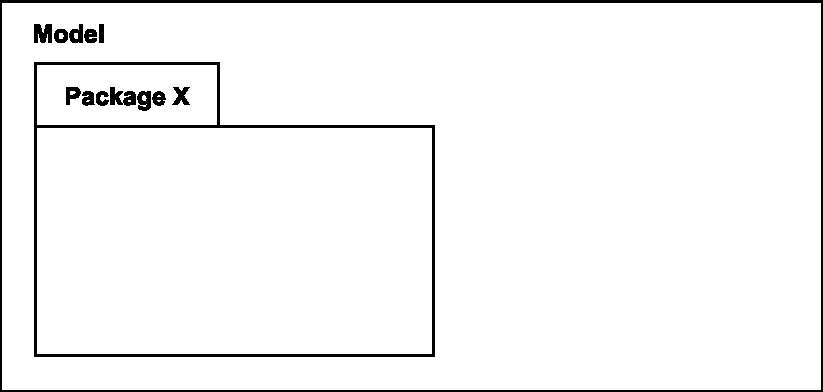
\includegraphics[width=\linewidth]{images/illustration_1}
        \caption{Initial state}
        \label{fig:illustration_1}
    \end{subfigure}
    \begin{subfigure}[t]{0.245\linewidth}
        \centering
        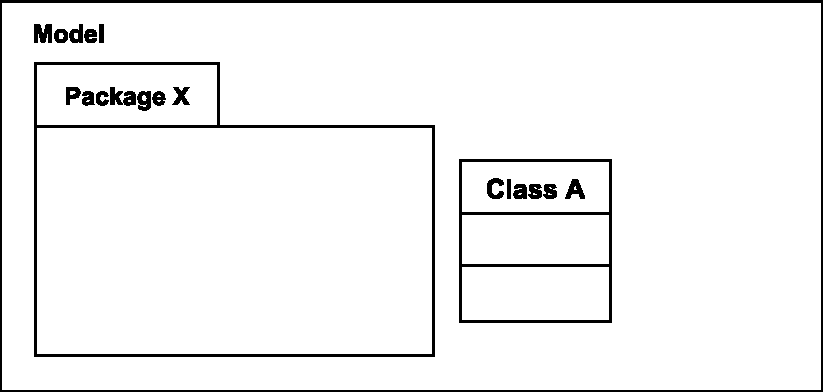
\includegraphics[width=\linewidth]{images/illustration_2}
        \caption{Time stamp 1}
        \label{fig:illustration_2}
    \end{subfigure}
    \begin{subfigure}[t]{0.245\linewidth}
        \centering
        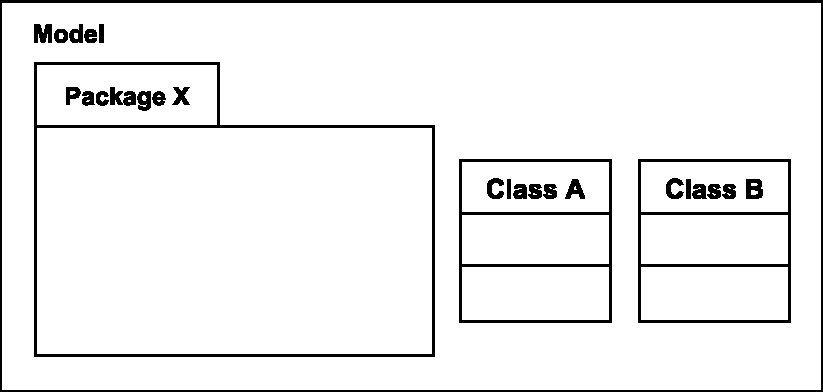
\includegraphics[width=\linewidth]{images/illustration_3}
        \caption{Time stamp 2}
        \label{fig:illustration_3}
    \end{subfigure}
    \begin{subfigure}[t]{0.245\linewidth}
        \centering
        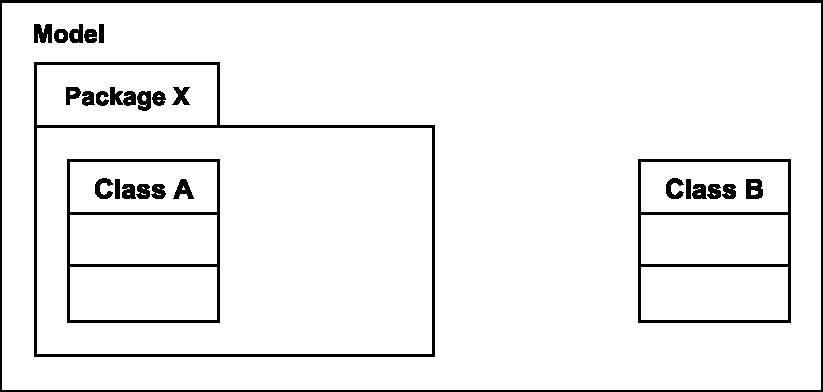
\includegraphics[width=\linewidth]{images/illustration_4}
        \caption{Time stamp 3}
        \label{fig:illustration_4}
    \end{subfigure}
    \hfill
    \begin{subfigure}[t]{0.245\linewidth}
        \centering
        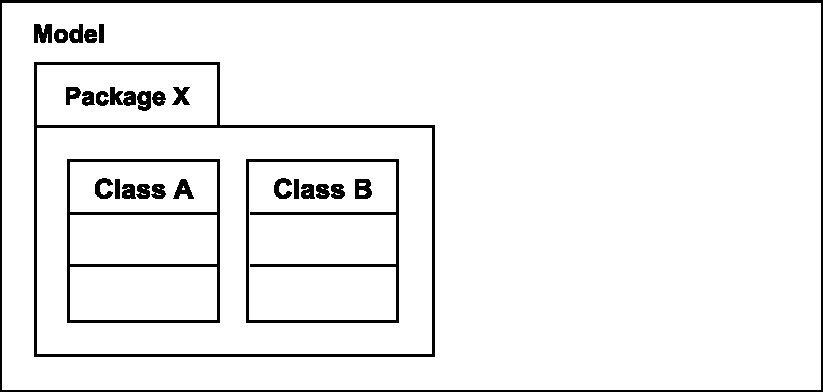
\includegraphics[width=\linewidth]{images/illustration_5}
        \caption{Time stamp 4}
        \label{fig:illustration_5}
    \end{subfigure}
    \begin{subfigure}[t]{0.245\linewidth}
        \centering
        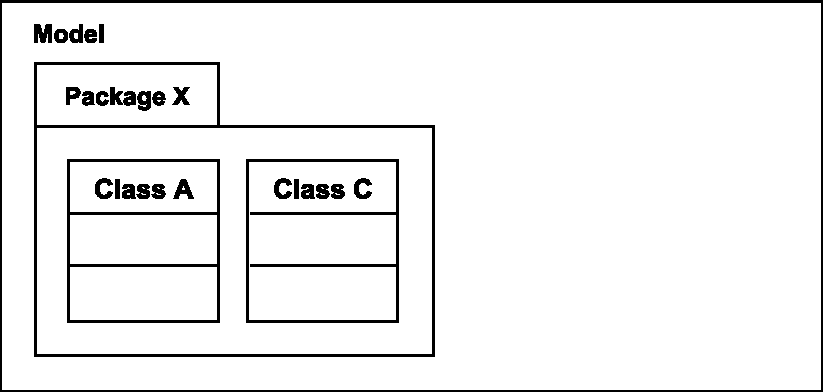
\includegraphics[width=\linewidth]{images/illustration_6}
        \caption{Time stamp 5}
        \label{fig:illustration_6}
    \end{subfigure}
    \begin{subfigure}[t]{0.245\linewidth}
        \centering
        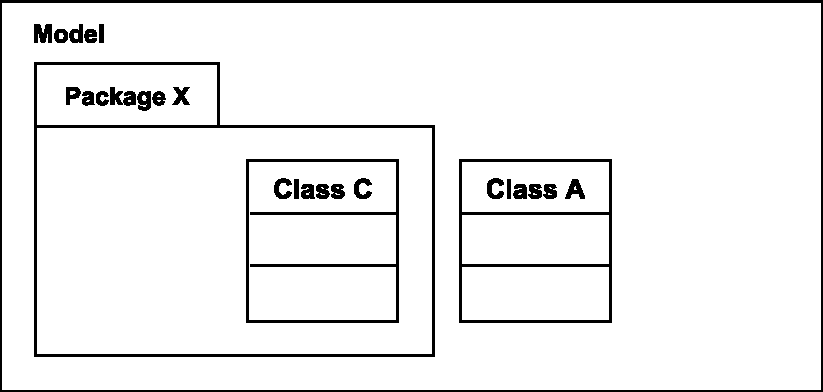
\includegraphics[width=\linewidth]{images/illustration_7}
        \caption{Time stamp 6}
        \label{fig:illustration_7}
    \end{subfigure}
    \begin{subfigure}[t]{0.245\linewidth}
        \centering
        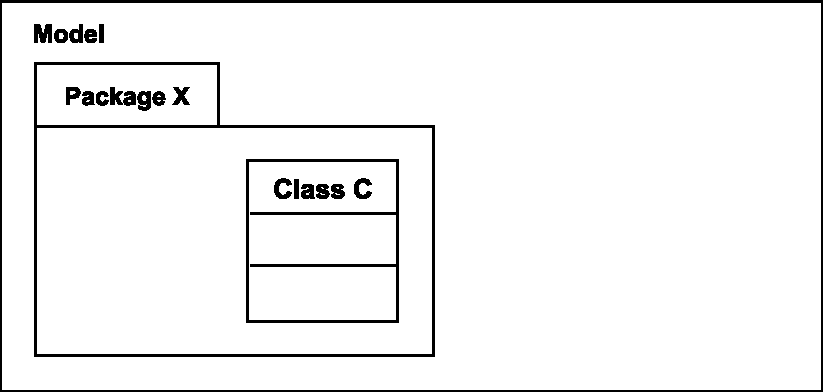
\includegraphics[width=\linewidth]{images/illustration_8}
        \caption{Time stamp 7}
        \label{fig:illustration_8}
    \end{subfigure}
    
    \caption{The states of the example model after certain changes and their corresponding lines in Listing \ref{lst:cbpmodel}.}
    \label{fig:illustration_cbp}
\end{figure}

To load an SBP model, only the elements that are in the final state need to be instantiated. To load a CBP model, all the events that lead to the final state must be replayed. Loading times for SBP models are proportional to the size of the model. Loading times for CBP models are proportional to the number of events. As a result, loading times of CBP models will always increase over time and are considerably longer than for SBP \cite{yohannis2018towards,mens2002state}. 

To store an SBP model, all the elements that exist in the final state must be persisted. To save a CBP, only the change events in the last session need to be persisted. Storing times of SBP models are proportional to the size of the model. Storing times of CBP models are proportional to the number of events in a session. As a result, storing times of CBP models can be considerably shorter than for SBP models \cite{yohannis2018towards}. %"Storing of CBP models also requires more space as events just keep adding up. " comes up in more detail in next para, so deleted here.

Comparing and finding the differences between two versions of a state-based model is expensive \cite{Kolovos:2009:DMM:1564596.1564641} ($O(N^2)$ in the general case) % \cite{}) operation and beyond 
which affects the efficiency of change visualisation and comprehension, and has a substantial impact on downstream activities such as incremental model transformation \cite{DBLP:conf/ecmdafa/OgunyomiRK15} and validation.

By contrast, in CBP, changes are first-class entities in the persisted model file and as such, model comparison and differencing is relatively inexpensive (Section \ref{sec:evaluation}). The main downsides of CBP are ever-growing model file sizes \cite{DBLP:journals/entcs/RobbesL07,DBLP:conf/edoc/KoegelHLHD10} and ever-increasing loading times \cite{mens2002state}. Loading times can be reduced by around 50\% by processing the changelog, detecting, memorising and subsequently ignoring change events that have no impact to the final state of the model, but are still substantially longer -- more than 6.4 times slower and even longer as the persisted changes increase -- than loading times for state-based approaches \cite{yohannis2018towards}. Table \ref{table:persistence_comparsion} summarises the benefits (+) and drawbacks (-) of change and state-based model persistence.

\section{Hybrid Model Persistence}
\label{sec:hybrid_model_persistence}
To achieve the best of both worlds we introduce a hybrid model persistence approach which combines change-based and state-based model persistence, to work together side-by-side. An overview of the proposed approach is illustrated in Fig. \ref{fig:hybrid_persistence}.

\begin{figure}[ht]
    \begin{subfigure}{0.49\linewidth}
        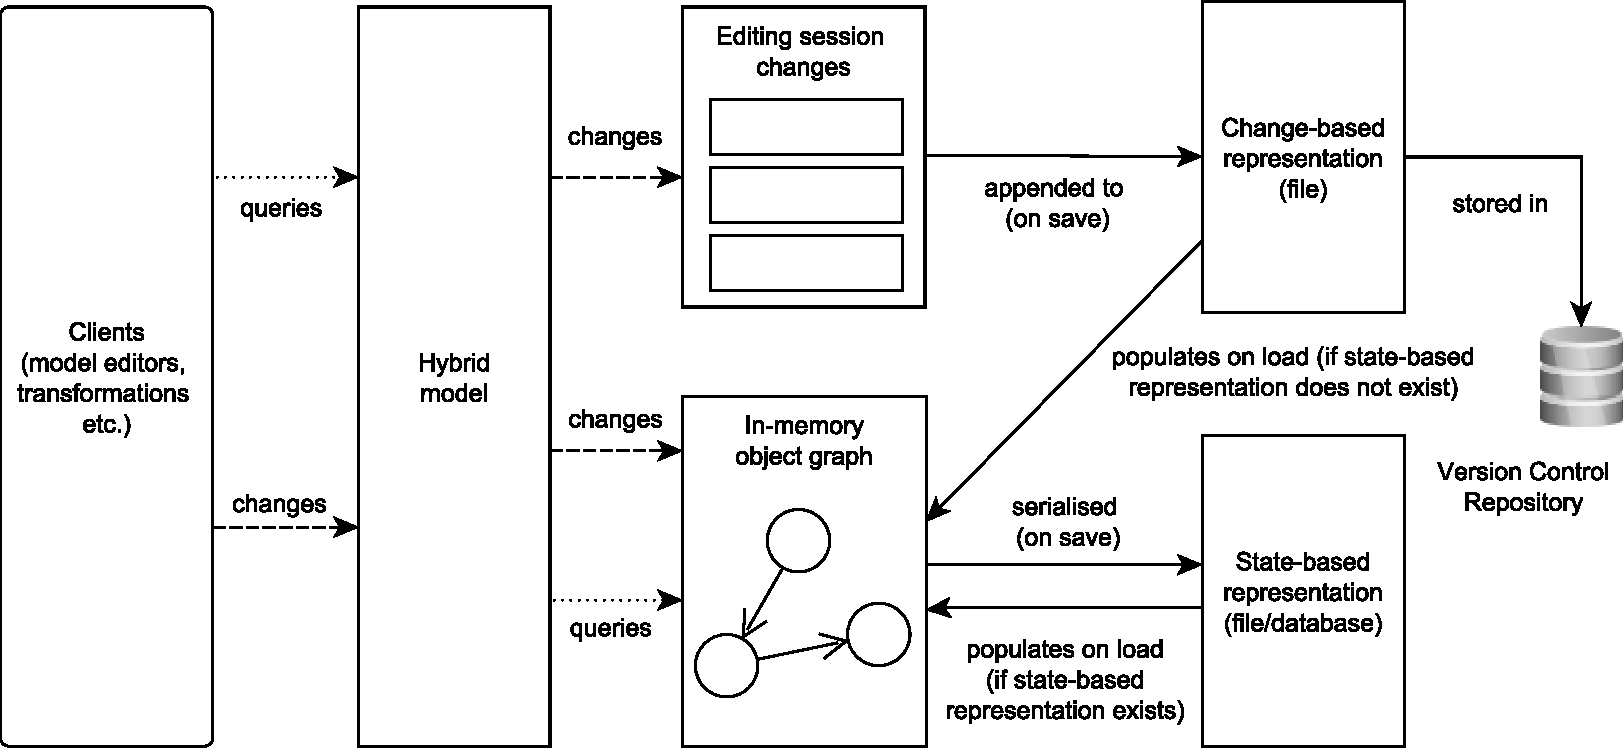
\includegraphics[width=\linewidth]{images/hybrid_persistence}
        \caption{The mechanism of hybrid model persistence.}
        \label{fig:hybrid_persistence}
    \end{subfigure}
    \begin{subfigure}{0.49\linewidth}
        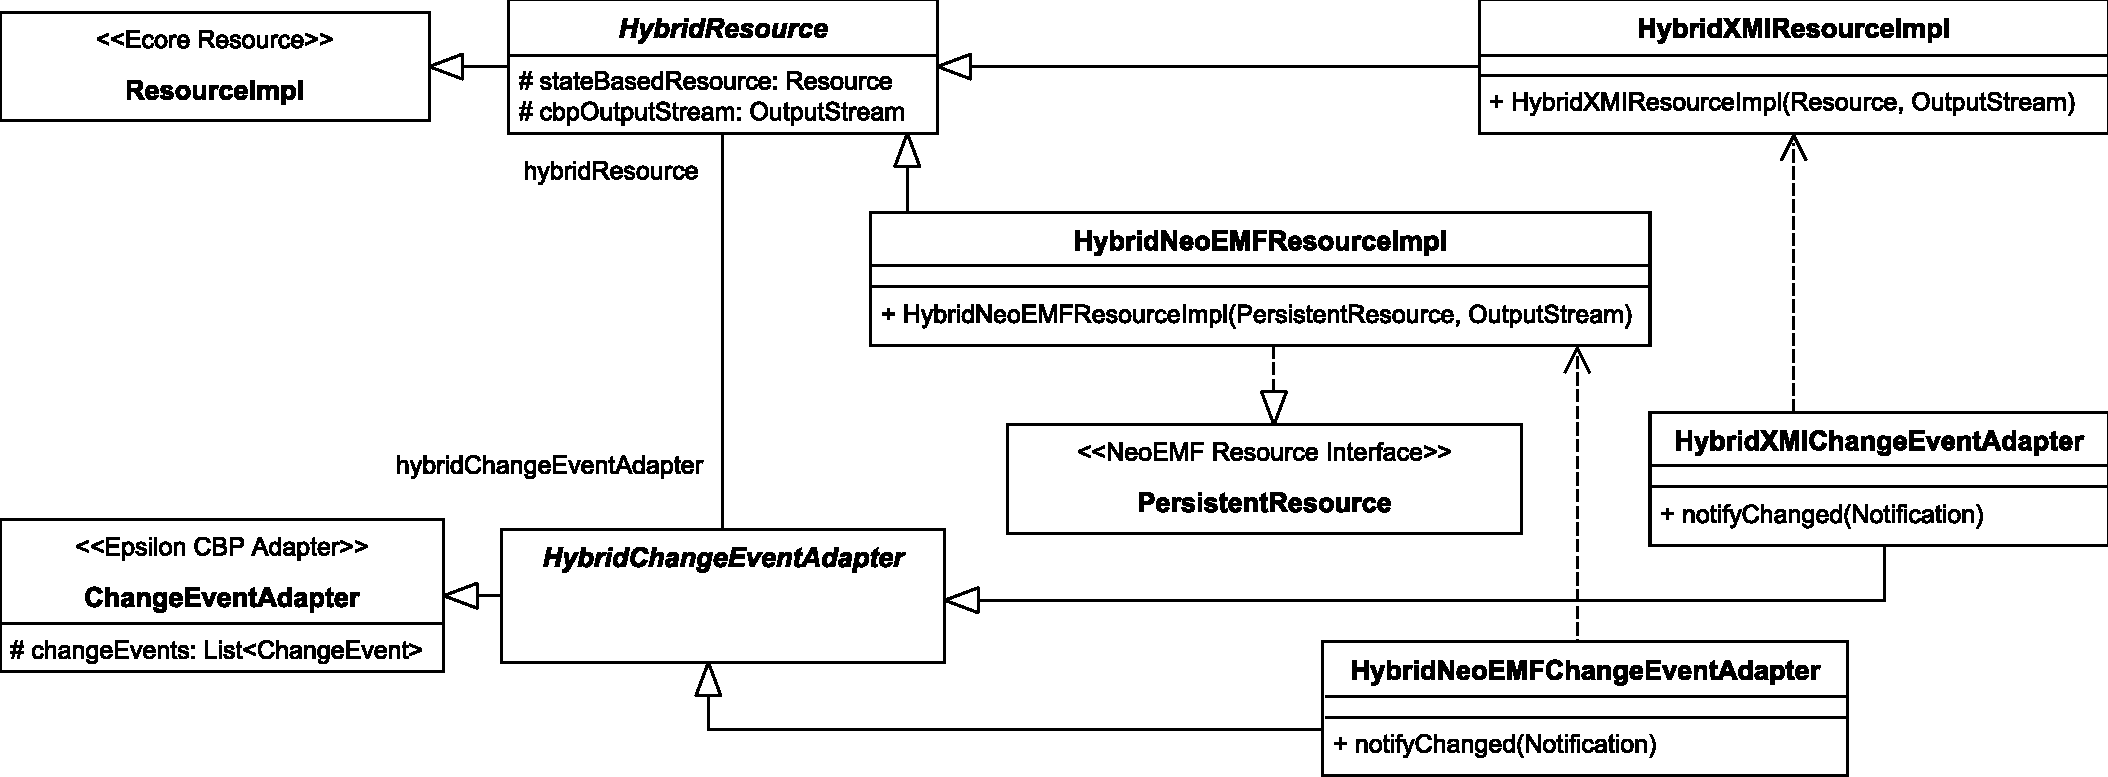
\includegraphics[width=\linewidth]{images/class_diagram}
        \caption{Class diagram showing the core components of the hybrid model persistence implementation.}
        \label{fig:class_diagram}
    \end{subfigure}
\end{figure}

In the proposed approach a \textit{hybrid} model is stored in two representations at the same time: a change-based (e.g. using CBP) and a state-based representation (e.g. using XMI or a database-backed approach such as NeoEMF). The change-based representation is the source of truth. The state-based representation can be fully derived from the change-based representation.

\textbf{Loading a hybrid model.} Models are loaded into in-memory object graphs that clients (e.g. editors, transformations) can then interact with\footnote{Depending on the state persistence mechanism, the object graph may be loaded in its entirety at startup (e.g. XMI) or loaded progressively, in a lazy manner (e.g. NeoEMF/CDO)}. In the proposed hybrid approach, if the state-based counterpart already exists, the in-memory object graph is populated from it; otherwise, it is populated by replaying the complete editing history recorded in the change-based representation.

\textbf{Changing a hybrid model.} When an element in a loaded model is created, modified or deleted, the change is applied to the in-memory object graph and is also recorded in an in-memory list of changes (\textit{Editing session changes} in Fig 2). We use the term \emph{editing session} for the period between loading a model and saving back to disk. 

\textbf{Saving a hybrid model.} The current version of the in-memory object graph is stored in the preferred state-based representation. The list of changes recorded in the current editing session (with optional processing, as described above) is appended to the change-based representation.

\textbf{Versioning a hybrid model.} Since the state-based representation is fully derived from the change-based representation, if a model needs to be versioned (e.g. in a Git repository), only the change-based representation needs to be stored. The first time it is loaded after being checked out/cloned, the state-based representation is computed and persisted locally and is used in subsequent model loading steps.

\textbf{Comparing hybrid models.} To compare two hybrid models, their change-based representations are used: this is much more efficient than state-based comparison as demonstrated in Section \ref{sec:change_detection}.

\section{Implementation}
\label{sec:implementation}

We have implemented the proposed hybrid model persistence approach in a prototype on top of the Eclipse Modeling Framework (EMF) \cite{steinberg2008emf}. The prototype makes use of an existing implementation of change-based model persistence, the Epsilon CBP \cite{DBLP:conf/models/YohannisKP17}, augmented with two state-based persistence implementations: NeoEMF \cite{daniel2016neoemf} and XMI \cite{omg2018xmi}.

XMI has been selected as a standard state-based model persistence format (natively supported by EMF), and NeoEMF as a best-of-breed representative of database-backed state-based model persistence frameworks. The core components of the prototype are presented in Fig. \ref{fig:class_diagram}. 

The Epsilon CBP provides a \textit{ChangeEventAdapter} class \cite{DBLP:conf/models/YohannisKP17} that extends from Ecore's \textit{EContentAdapter} adapter class \cite{eclipse2018eContentAdapter}. This class collects changes made to the in-memory object graph of an EMF model in the form of a list of events (\textit{changeEvents}). Based on this class, we derived an adapter class, \textit{ChangeHybridEventAdapter}, for the hybrid model persistence implementation. It is an abstract class so that it can be further derived to create different implementations of adapter classes for different types of state-based persistence. The \textit{ChangeHybridNeoEMFEventAdapater} is the adapter class for NeoEMF, and the \textit{ChangeHybridXMIEventAdapater} for XMI. These classes override \textit{notifyChanged}(\textit{Notification}) in the \textit{ChangeEventAdapter} class, to handle events that are specific to NeoEMF and XMI, respectively.

We also created a resource class for hybrid persistence, \textit{HybridResource} (a resource class is a class dedicated to interacting with a persistence, e.g. save, load, get contents), derived from the Ecore's \textit{ResourceImpl} \cite{eclipse2018resourceImpl}. The class is again abstract so that it can be realised in different resource implementation classes for different state-based persistence. The \textit{HybridResource} class contains the \textit{stateBasedResource} field which is used to refer to a state-based persistence that is being used, and the \textit{cbpOutputStream} field that refers to an \textit{OutputStream} (e.g. file, in-memory) as the representation of the CBP for saving changes. \textit{HybridResource} has an association with \textit{HybridChangeEventAdapater}, so that the former can access the events collected by the latter, and the latter can also use facilities provided by the former (e.g. getting the identity of an element in the resource; saving changes to a change-based model representation).

The resource implementation classes for NeoEMF and XMI are \textit{HybridNeoEMFResourceImpl} and \textit{HybridXMIResourceImpl} respectively. \textit{HybridNeoEMFResourceImpl} also implements the NeoEMF's \textit{PersistenceResource} interface \cite{atlanmod2018persistentResource} so that specific NeoEMF's methods can be used (e.g. \textit{close}(), to close a connection with a backend database). The complete implementation is available under
%[Hidden for Blind Review].
\url{https://github.com/epsilonlabs/emf-cbp}.

\subsection{Known Limitations}


Our prototype supports all the core constructs of Ecore, including classes, inheritance, single or multi-valued attributes and references, datatypes and containment. It also supports session-based changes to models that are atomic editor events, such as creating and deleting an object, setting and unsetting a feature. 

With regard to notable limitations, the hybrid model persistence can only support single-file models: fragmented across multiple files and cross-model references models persisted in more than one file or backend. Secondly, an assumption is made that the two underpinning representations (change-based and state-based) are always consistent with each other, i.e. that they are always modified as an indivisible unit.

\section{Evaluation}
\label{sec:evaluation}

In this section, we compare hybrid model persistence (Epsilon CBP with each of NeoEMF and XMI) vs. state-based persistence (NeoEMF or XMI only) on loading, saving, and storage space usage,
and demonstrate that hybrid model persistence offers the best of both worlds: fast model loading and saving, and efficient change detection. The data used in the evaluation are available under
%[hidden for review]
\url{https://goo.gl/hRnpbo}.


\subsection{Evaluation Method}
\label{sec:evaluation_method}
%"We developed the prototype of the proposed hybrid model persistence approach. " removed as it is obvious, later and in the footnote now above, that this is what you are reporting on.

The evaluation was performed on Intel\textsuperscript{\textregistered} Core\textsuperscript{TM} i7-6500U CPU @ 2.50GHz 2.59GHz, 12GB RAM, and the Java\textsuperscript{TM} SE Runtime Environment (build 1.8.0\textunderscore162-b12).

For the evaluation, we used models reverse-engineered from the Java source code of a real-world open-source project (Epsilon \cite{eclipse2017epsilon,eclipse2018epsilongit}). For state-based representation of the models, we used the MoDisco tool \cite{DBLP:journals/infsof/BruneliereCDM14} to generate XMI-based UML2 \cite{eclipse2017uml2} models that reflect the classes, fields, and operation signatures of the source code of the project and then imported the generated models into NeoEMF. We also derived UML2 models for BPMN2 \cite{eclipse2017bpmn2} and MoDiscoXML models (models that conforms to the generic XML metamodel as provided by MoDisco) \cite{eclipse2018modiscoxml} from the Wikipedia article on the United States \cite{wikipedia2018us}. % The source for this paragraph is not in git, so I have typed it in, with simplifications! You need to add back in the citations!

Reverse-engineering a state-based representation of a model is trivial; the change-based representing is more challenging. Here, a change-based representation was derived from the diffs identified from the subsequent versions of the Java source code committed on its Git repository. The change-based representation was derived by comparing an initially-empty running model to the generated models sequentially, ordered by their versions. All identified differences were then reconciled by performing a one-way merge to the running model. All changes made to the running model during the merging process were captured and persisted into a CBP file. The comparison and merging were performed using EMF Compare \cite{eclipse2017compare}. This procedure follows the procedure performed in \cite{yohannis2018towards}. %This sentence is moved from earlier, but is not in the repository text: again you need to re-add the citation.

Using these models, we evaluate the performance of our hybrid persistence prototype against XMI and NeoEMF in terms of time and memory footprint for loading, saving, and comparison/diffing of subsequent model versions using EMF Compare was used the baseline for the state-based comparison. %For the latter, we measured the delta of memory used before and after loading and saving completes. We also measured the impact of using the hybrid approach on the execution time of a model comparison, specifically for identifying differences between a model and its preceding version. The hybrid approach was compared to model-to-model comparison using EMF Compare on their execution time.

We repeated our experiments 22 times for each dimension measured. Since the data were not normally distributed, we used the nonparametric Mann-Whitney U test \cite{doi:10.1002/9780470479216.corpsy0524} with a significance level of 5\%.

. % If t-test' $p$-$value$ $<$ 0.05, we rejected the null hypothesis -- the $means$ of the compared persistence types are equal ($H_0$) -- and accepted the alternative hypothesis -- the $means$ of the compared persistence types are not equal ($H_1$). 

%\textbf{F: not convinced that the data you have is suitable for a t-test (which has many many required data characteristics) but this is not the right place to change. Think about a non-parametric statistic to compare mean in the thesis... also check that means and medians are similar (i.e. the data is not skewed); if they are not similar you MUST use a comparison of medians (e.g. the A test). I've cursorily checked that your results are not going to be way out because you used a silly statistic! }

\subsection{Loading Time and Memory Footprint}
\label{sec:model_loading_time}
In this section, we present the results of our evaluation on the time and memory footprint required for the hybrid model persistence to load a model. In the following plots, we use the XMI and NEO labels for out-of-the-box XMI and NeoEMF and the H-XMI and H-NEO labels for our hybrid persistence prototypes based on XMI and NeoEMF.

\subsubsection{Epsilon Project.}
\label{sec:model_loading_time_epsilon}
The model used for testing is the UML2 model of the Epsilon project that consists of 88,020 elements. The model is derived from the committed version number 940 from its Git repository \cite{eclipse2018epsilongit}. 

The results show that the average loading time using Hybrid NeoEMF ($mean$ = 0.292, $sd$ = 0.061 seconds) is slightly slower than NeoEMF ($mean$ = 0.279, $sd$ = 0.023 seconds) but insignificant ($W$ = 258, $p$-value = 0.72). For Hybrid XMI, the slowdown is significant ($W$ = 26, $p$-value $<$ 0.05), hybrid XMI taking ($mean$ = 0.=317, $sd$ = 0.006 seconds), compared to XMI ($mean$ = 0.270, $sd$ = 0.018 seconds). As a reference, we also measured the time required for the optimised CBP loading approach in \cite{yohannis2018towards} to load the model. The time required to load the model is $mean$ = 16.96, $sd$ = 1.26 seconds, which is clearly outperformed the by the other persistence approaches (see Table \ref{table:space_usage} for the number of events contained by the CBP).

The memory footprint after loading the model for Hybrid NeoEMF ($mean$ = 38.601, $sd$ = 0.878 MBs) is larger than for NeoEMF ($mean$ = 10.014, $sd$ = 1.088 MBs); the result is statistically significant ($W$ = 0, $p$-value $<$ 0.05). A similarly significant increase of the memory footprint ($W$ = 0, $p$-value $<$ 0.05) is found when comparing Hybrid XMI ($mean$ = 10.72018, $sd$ = 0.00022 MBs) and XMI ($mean$ = 10.72009, $sd$ = 0.00024 MBs) when loading the model. 

\begin{figure}[ht]
    \begin{subfigure}{0.49\linewidth}
        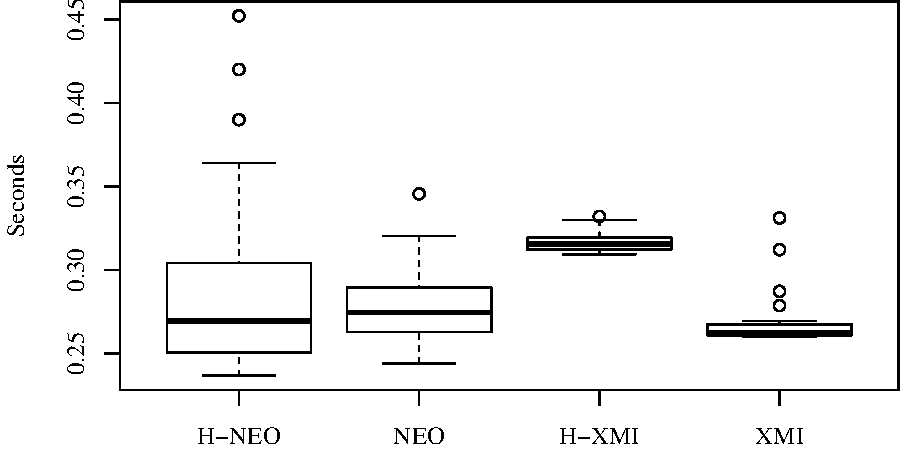
\includegraphics[width=\linewidth]{images/load_time_epsilon}
        \caption{loading time}
        \label{fig:load_time_epsilon}
    \end{subfigure}
    \begin{subfigure}{0.49\linewidth}
        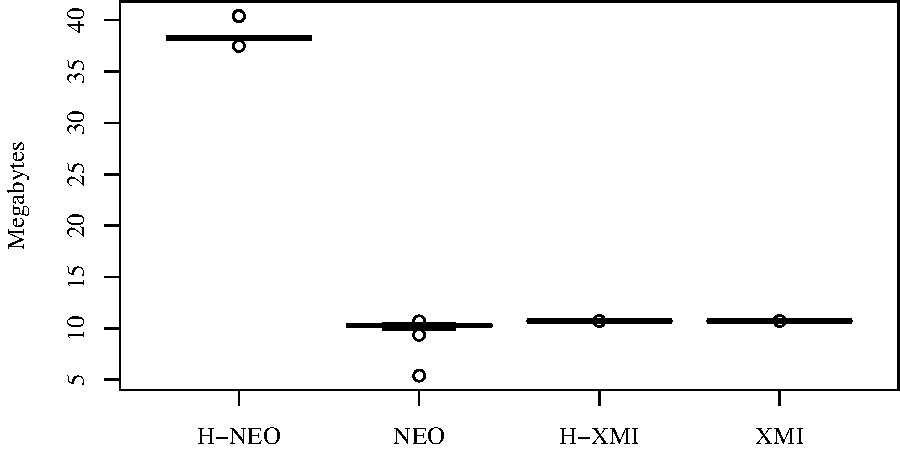
\includegraphics[width=\linewidth]{images/load_memory_epsilon}
        \caption{loading memory footprint}
        \label{fig:load_memory_epsilon}
    \end{subfigure}
\caption{Hybrid vs. state-based model persistence for the Epsilon project.}
\end{figure}

\subsubsection{BPMN2 Project.}
\label{sec:model_loading_time_bpmn2}
The UML2 model of the BPMN2 project consists of 62,062 elements. The model is derived from the committed version number 192 from its Git repository \cite{eclipse2018bpmn2git}. 

For this model, the average loading time for Hybrid NeoEMF ($mean$ = 0.308, $sd$ = 0.071 seconds) is slightly slower than for NeoEMF ($mean$ = 0.286, $sd$ = 0.025 seconds) but the result is not significant ($W$ = 230, $p$-value = 0.79). The slowdown is statistically significant ($W$ = 37, $p$-value $<$ 0.05) for Hybrid XMI ($mean$ = 0.212, $sd$ = 0.016 seconds) vs.compared to XMI ($mean$ = 0.179, $sd$ = 0.016 seconds). As a reference, the optimised CBP \cite{yohannis2018towards} takes $mean$ = 3.97, $sd$ = 0.02 seconds to load the model, which is slower than the other persistence approaches (see Table \ref{table:space_usage} for the number of events contained by the CBP). 

For the memory footprint after loading the model, Hybrid NeoEMF ($mean$ = 40.78, $sd$ = 1.29 MBs) uses more memory than NeoEMF ($mean$ = 27.20, $sd$ = 1.05 MBs); the result is statistically significant ($W$ = 0, $p$-value $<$ 0.05). For the comparison between Hybrid XMI ($mean$ = 6.73374, $sd$ = 1.29305 MBs) and XMI ($mean$ = 6.73367, $sd$ = 0.00056 MBs), the increase of memory footprint is also significant ($W$ = 101, $p$-value $<$ 0.05). 

\begin{figure}[ht]
    \begin{subfigure}{0.49\linewidth}
        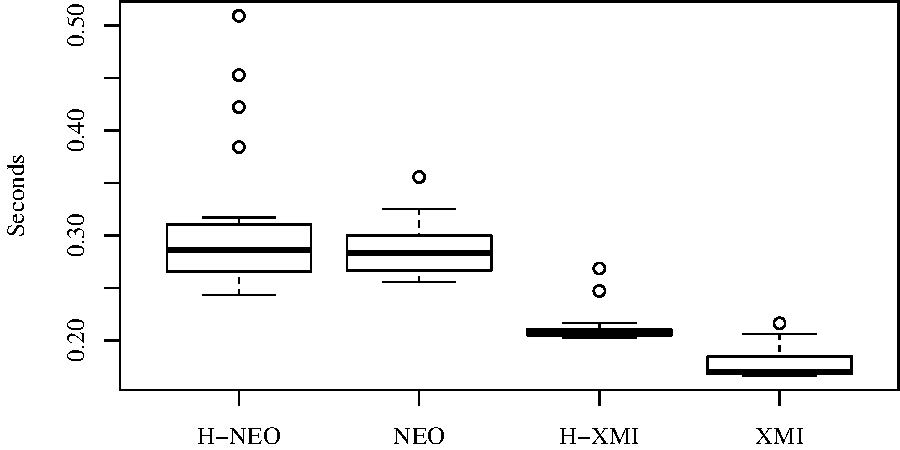
\includegraphics[width=\linewidth]{images/load_time_bpmn2}
        \caption{loading time}
        \label{fig:load_time_bpmn2}
    \end{subfigure}
    \begin{subfigure}{0.49\linewidth}
        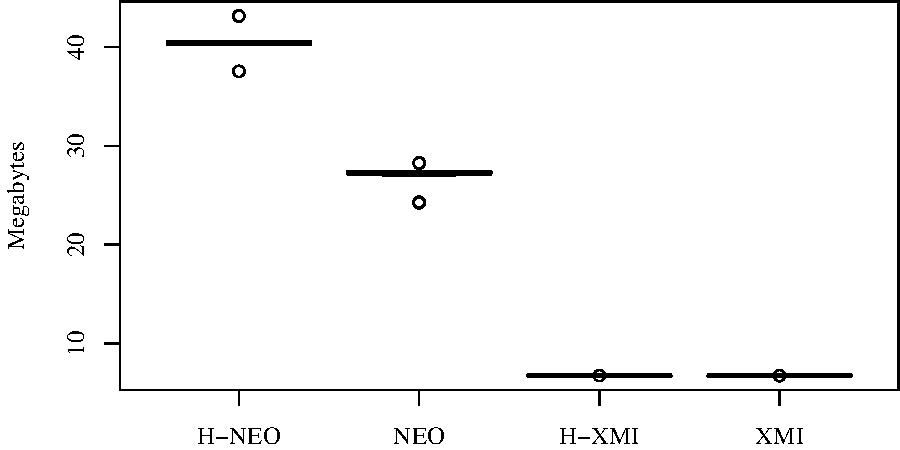
\includegraphics[width=\linewidth]{images/load_memory_bpmn2}
        \caption{loading memory footprint}
        \label{fig:load_memory_bpmn2}
    \end{subfigure}
\caption{Hybrid vs. state-based model persistence for the BPMN2 project.}
\end{figure}

\subsubsection{Wikipedia Article.}
\label{sec:model_loading_time_wikipedia}

The ModiscoXML model of the Wikipedia's United States article consists of 13,122 elements. The model is derived from the version number 10,187 (id 45118452) of its online page \cite{wikipedia2018us}. 

For this model, the average loading time of Hybrid NeoEMF ($mean$ = 0.262, $sd$ = 0.048 seconds) is slightly faster than NeoEMF ($mean$ = 0.273, $sd$ = 0.062 seconds) but insignificant ($W$ = 250, $p$-value $<$ 0.86). The slowdown on Hybrid XMI ($mean$ = 0.045, $sd$ = 0.001 seconds) compared to XMI ($mean$ = 0.040, $sd$ = 0.001 seconds) is also significant ($W$ = 0, $p$-value $<$ 0.05). As a reference, the optimised CBP \cite{yohannis2018towards} requires $mean$ = 228.83, $sd$ = 6.59 seconds to load the model, which is very slow compared to the other persistence approaches (see Table \ref{table:space_usage} for the number of events contained by the CBP). 

For the memory footprint after loading the model, Hybrid NeoEMF ($mean$ = 35.91, $sd$ = 1.03 MBs) uses more memory than NeoEMF ($mean$ = 27.25, $sd$ = 0.54 MBs); the difference is statistically significant ($W$ = 0, $df$ = $p$-value $<$ 0.05). A significant difference ($W$ = 0, $p$-value $<$ 0.05) is also found when comparing the memory footprint for Hybrid XMI ($mean$ = 8.4079, $sd$ = 0.0008 MBs) vs. XMI ($mean$ = 8.0933, $sd$ = 0.0009 MBs). 

\begin{figure}[ht]
    \begin{subfigure}{0.49\linewidth}
        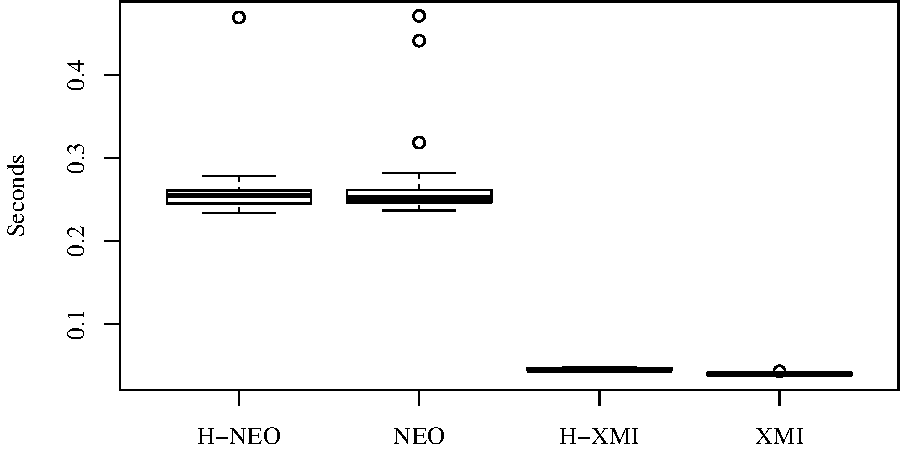
\includegraphics[width=\linewidth]{images/load_time_wikipedia}
        \caption{loading time}
        \label{fig:load_time_wikipedia}
    \end{subfigure}
    \begin{subfigure}{0.49\linewidth}
        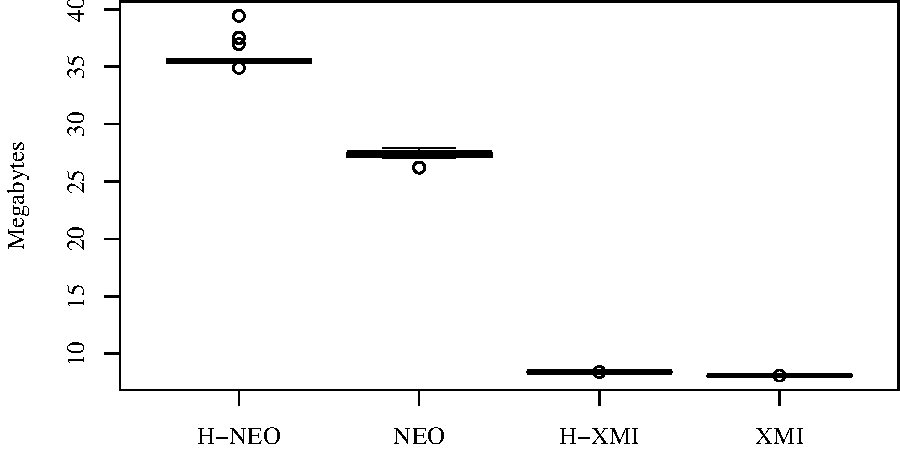
\includegraphics[width=\linewidth]{images/load_memory_wikipedia}
        \caption{loading memory footprint}
        \label{fig:load_memory_wikipedia}
    \end{subfigure}
\caption{Hybrid vs. state-based model persistence for the Wikipedia article.}
\end{figure}

\subsection{Model Saving Time and Memory Footprint}
\label{sec:model_saving_time}

In this section, we evaluated the time taken to save a changed model using hybrid model persistence, and the change in memory footprint. The models are the same as those used in Section \ref{sec:model_loading_time}.

\subsubsection{Epsilon Project.}
\label{sec:model_saving_time_epsilon}
For UML2 model version 940 of the Epsilon project, the average Hybrid NeoEMF saving time for each change ($mean$ = 0.0892, $sd$ = 0.0421 seconds) is slightly slower than for NeoEMF ($mean$ = 0.0829, $sd$ = 0.0494 seconds) and the difference is not statistically significant ($W$ = 216, $p$-value = 0.55). The slowdown is statistically significant ($W$ = 78, $p$-value $<$ 0.05) for Hybrid XMI ($mean$ = 0.411, $sd$ = 0.023 seconds) vs. XMI ($mean$ = 0.397, $sd$ = 0.015 seconds). 

The memory footprint after saving a change to the model in Hybrid NeoEMF ($mean$ = 2.64, $sd$ = 1.29 MBs) is larger than for NeoEMF ($mean$ = 2.61, $sd$ = 0.78 MBs) but is not statistically significant ($W$ = 283, $p$-value $=$ 0.34). The Hybrid XMI ($mean$ = 1.56355, $sd$ = 0.0005 MBs) also uses more memory than XMI ($mean$ = 1.56326, $sd$ = 0.0018 MBs) when loading the model and also significant ($W$ = 408, $p$-value $<$ 0.05). 

\begin{figure}[ht]
    \begin{subfigure}{0.49\linewidth}
        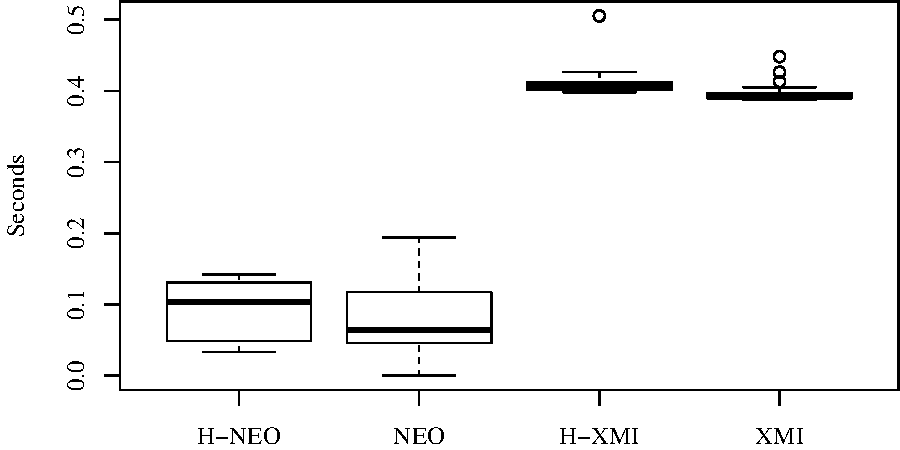
\includegraphics[width=\linewidth]{images/save_time_epsilon}
        \caption{saving time}
        \label{fig:save_time_epsilon}
    \end{subfigure}
    \begin{subfigure}{0.49\linewidth}
        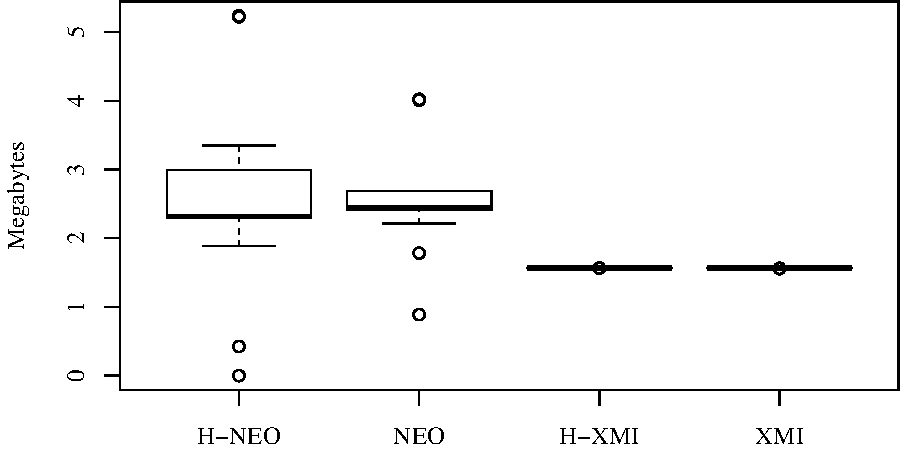
\includegraphics[width=\linewidth]{images/save_memory_epsilon}
        \caption{saving memory footprint}
        \label{fig:save_memory_epsilon}
    \end{subfigure}
\caption{Hybrid vs. state-based model persistence for the Epsilon project.}
\end{figure}

\subsubsection{BPMN2 Project.}
\label{sec:model_saving_time_bpmn2}
For the UML2 model version 192 of the BPMN2 project, the average saving time for each change using Hybrid NeoEMF ($mean$ = 0.0777, $sd$ = 0.0424 seconds) is slightly slower than the for NeoEMF ($mean$ = 0.0775, $sd$ = 0.0452 seconds) but not statistically significant ($W$ = 213, $p$-value = 0.51). The slowdown is statistically significant ($0$ = 0, $p$-value $<$ 0.05) for Hybrid XMI ($mean$ = 0.33, $sd$ = 0.007 seconds) vs. XMI ($mean$ = 0.28, $sd$ = 0.008 seconds). 

The memory footprint after saving a change made to the model in Hybrid NeoEMF ($mean$ = 1.86, $sd$ = 3.86 MBs) is larger than for NeoEMF ($mean$ = 1.52, $sd$ = 0.77 MBs) but not significant ($W$ = 308, $p$-value $<$ 0.12). Hybrid XMI ($mean$ = 0.8378, $sd$ = 0.00361 MBs) also uses more memory than XMI ($mean$ = 0.8375, $sd$ = 0.00362 MBs) when loading the model and at the significant level ($W$ = 58, $p$-value $<$ 0.05). 

\begin{figure}[ht]
    \begin{subfigure}{0.49\linewidth}
        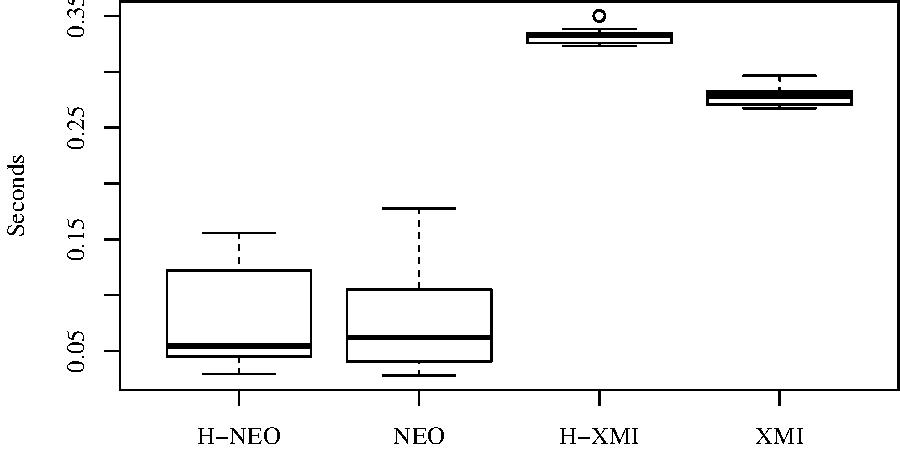
\includegraphics[width=\linewidth]{images/save_time_bpmn2}
        \caption{saving time}
        \label{fig:save_time_bpmn2}
    \end{subfigure}
    \begin{subfigure}{0.49\linewidth}
        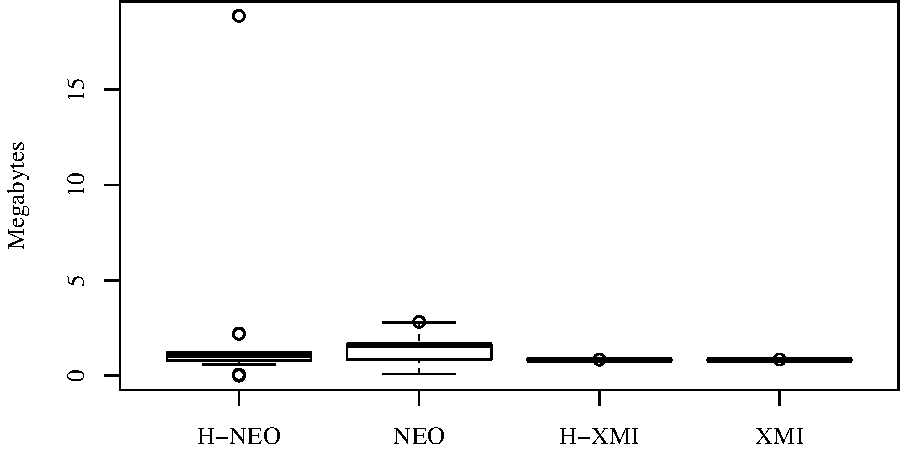
\includegraphics[width=\linewidth]{images/save_memory_bpmn2}
        \caption{saving memory footprint}
        \label{fig:save_memory_bpmn2}
    \end{subfigure}
\caption{Hybrid vs. state-based model persistence for the BPMN2 project.}
\end{figure}

\subsubsection{Wikipedia Article.}
\label{sec:model_saving_time_wikipedia}
The MoDiscoXML model version 10,187 of the Wikipedia's United States article has an average saving time for each change in Hybrid NeoEMF ($mean$ = 0.135, $sd$ = 0.048 seconds) that is slightly slower than for NeoEMF ($mean$ = 0.120, $sd$ = 0.024 seconds) but the difference is not statistically significant ($W$ = 218, $p$-value = 0.59). The slowdown on Hybrid XMI ($mean$ = 0.024, $sd$ = 0.048 seconds) vs. XMI ($mean$ = 0.020, $sd$ = 0.002 seconds) is significant ($W$ = 42, $p$-value $<$ 0.05).

The memory footprint after saving a change made to the model using Hybrid NeoEMF ($mean$ = 1.32, $sd$ = 1.51 MBs) is larger than for NeoEMF ($mean$ = 0.97, $sd$ = 0.76 MBs) but statistically insignificant ($W$ = 189, $p$-value $=$ 0.22). Hybrid XMI ($mean$ = 0.0010, $sd$ = 0.00044 MBs) also uses more memory than XMI ($mean$ = 0.0005, $sd$ = 0.00001 MBs); the difference is significant ($W$ = 0, $p$-value $<$ 0.05). 

\begin{figure}[ht]
    \begin{subfigure}{0.49\linewidth}
        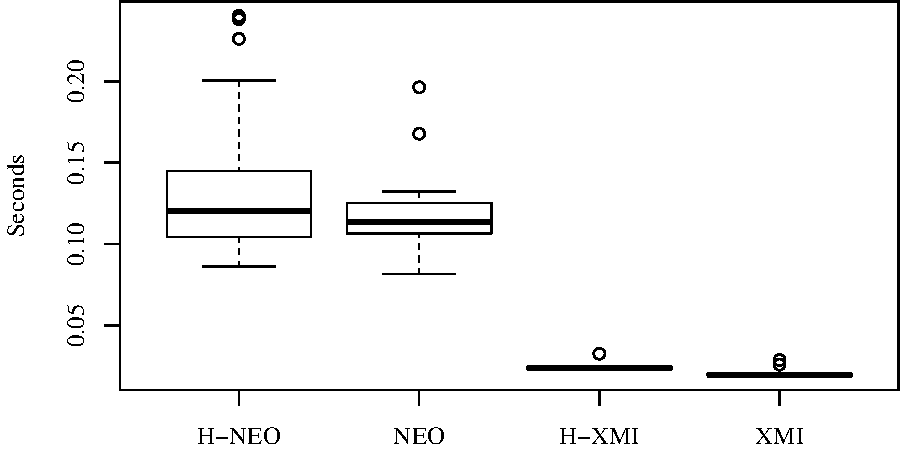
\includegraphics[width=\linewidth]{images/save_time_wikipedia}
        \caption{saving time}
        \label{fig:save_time_wikipedia}
    \end{subfigure}
    \begin{subfigure}{0.49\linewidth}
        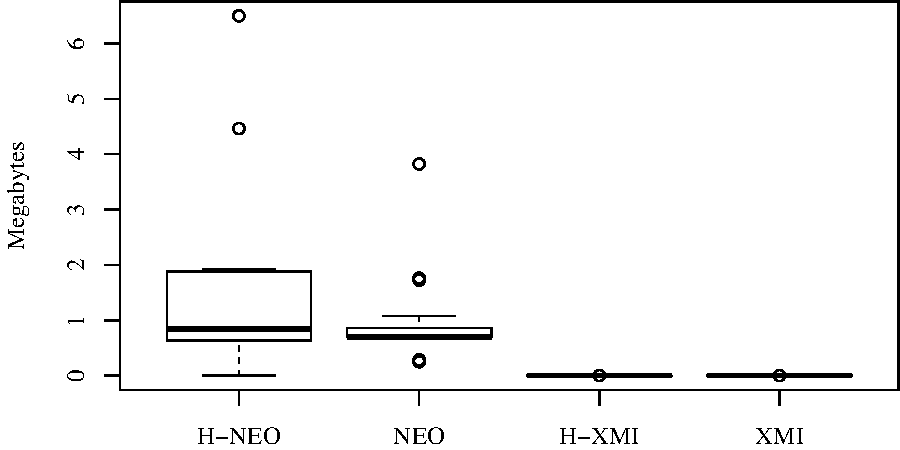
\includegraphics[width=\linewidth]{images/save_memory_wikipedia}
        \caption{saving memory footprint}
        \label{fig:save_memory_wikipedia}
    \end{subfigure}
\caption{Hybrid vs. state-based model persistence for the Wikipedia article.}
\end{figure}

\subsection{Storage Space Usage}
\label{sec:storage_space_usage}

To further evaluate storage space usage of the hybrid model persistence, we used the CBPs generated from the Epsilon project, the BPMN2 project, and the Wikipedia United States (US) article. We again generated the committed versions of the BPMN2 project as UML2 models and the versions of the Wikipedia article as MoDiscoXML models. For the Epsilon project, we have successfully generated CBPs from version 1 up to version 940. For the BPMN2 project and Wikipedia article, we have successfully generated their CBPs up to version number 192 and 10,187 respectively. The details (element count, event count, space size, and average space size per element or event) of their models when persisted in XMI, NeoEMF, and CBP are shown in Table \ref{table:space_usage}. 

The last column of each table derives an average space usage per element (for the SBPs) or event (for the CBP). We can estimate the storage space usage for a hybrid model persistence to be the combination of CBP and the appropriate SBP space usage.


\begin{table} [ht]
\centering
\begin{footnotesize}
\caption{Space usage for the Epsilon and BPMN2 projects, and the Wikipedia's United States article.}
\begin{tabular}{ | c | c | c | c | c | c | c | c | c | }
\hline
\multirow{2}{*}{Dimension} & \multirow{2}{*}{Case} & \multirow{2}{*}{Backend} & \multicolumn{2}{c|}{Hybrid} & \multicolumn{2}{c|}{Non-Hybrid} & \multicolumn{2}{c|}{Significance} \\
\hhline{~~~------}
& & & $mean$ & $sd$ & $mean$ & $sd$ &  $W$ & $p$-$value$ \\
\hline
%----------------
\multirow{6}{*}{\makecell{Loading\\Time}} & \multirow{2}{*}{Epsilon} & NeoEMF & 0.292 & 0.061 & 0.279 & 0.023 & 258 & \textbf{0.72}\\ 
\hhline{~~-------}
 & & XMI & 0.317 & 0.006 & 0.270 & 0.018 & 26 & $<$ 0.05 \\
 \hhline{~--------}
&\multirow{2}{*}{BPMN2} & NeoEMF & 0.308 & 0.071 &0.286 & 0.025 & 230 & \textbf{0.79}\\ 
\hhline{~~-------}
& & XMI & 0.212 & 0.016 & 0.179 & 0.016 & 37 & $<$ 0.05 \\
 \hhline{~--------}
&\multirow{2}{*}{Wikipedia}  & NeoEMF & 0.262 & 0.048 & 0.273 & 0.062 & 250 & \textbf{0.86}\\ 
\hhline{~~-------}
& & XMI & 0.045 & 0.001 & 0.040 & 0.001 & 0 & $<$ 0.05 \\
\hline
%--------------------

\multirow{6}{*}{\makecell{Loading\\Memory\\Footprint}} & \multirow{2}{*}{Epsilon} & NeoEMF & 38.601 & 0.878 & 10.014 & 1.088 & 0 & $<$ 0.05\\ 
\hhline{~~-------}
& & XMI & 10.72018 & 0.00022 & 10.72009 &0.00024 & 0 & $<$ 0.05 \\
\hhline{~--------}
&\multirow{2}{*}{BPMN2} & NeoEMF & 40.78 & 1.29 & 27.20 & 1.05 & 0 & $<$ 0.05\\ 
\hhline{~~-------}
& & XMI & 6.73367 & 1.29305 & 6.73367 & 0.00056 & 101 & $<$ 0.05 \\
\hhline{~--------}
&\multirow{2}{*}{Wikipedia}  & NeoEMF & 35.91 & 1.03 & 27.25 & 0.54 & 27.25 & \textbf{0.54}\\ 
\hhline{~~-------}
& & XMI & 8.4079 & 0.0008 & 8.0933 & 0.0009 & 0 & $<$ 0.05 \\
\hline
%--------------------

\multirow{6}{*}{\makecell{Saving\\Time}} & \multirow{2}{*}{Epsilon} & NeoEMF & 0.0892 & 0.0421 & 0.0829 & 0.0494 & 216 & \textbf{0.55}\\ 
\hhline{~~-------}
& & XMI & 0.411 & 0.023 & 0.397 & 0.015 & 78 & $<$ 0.05 \\
\hhline{~--------}
&\multirow{2}{*}{BPMN2} & NeoEMF & 0.0777 & 0.0424 & 0.0775 & 0.0452 & 213 & \textbf{0.51}\\ 
\hhline{~~-------}
& & XMI & 0.33 & 0.007 & 0.28 & 008 & 0 & $<$ 0.05 \\
\hhline{~--------}
&\multirow{2}{*}{Wikipedia} & NeoEMF & 0.135 & 0.048 & 0.120 & 0.024 & 218 & \textbf{0.59}\\ 
\hhline{~~-------}
& & XMI & 0.024 & 0.048 & 0.020 & 0.002 & 42 & $<$ 0.05 \\
\hline
%--------------------

\multirow{6}{*}{\makecell{Saving\\Memory\\Footprint}} & \multirow{2}{*}{Epsilon} & NeoEMF & 2.64 & 1.29 & 2.61 & 0.78 & 283 & \textbf{0.34}\\ 
\hhline{~~-------}
& & XMI & 1.56355 & 0.0005 & 1.56326 & 0.0018 & 408 & $<$ 0.05 \\
\hhline{~--------}
&\multirow{2}{*}{BPMN2} & NeoEMF & 1.86 & 3.86 & 1.52 & 0.77 & 308 & \textbf{0.12}\\ 
\hhline{~~-------}
& & XMI & 0.8378 & 0.00361 & 0.8375 & 0.00362 & 58 & $<$ 0.05 \\
\hhline{~--------}
&\multirow{2}{*}{Wikipedia}  & NeoEMF & 1.32 & 1.51 & 0.97 & 0.76 & 189 & \textbf{0.22}\\ 
\hhline{~~-------}
& & XMI & 0.0010 & 0.00044 & 0.0005 & 0.00001 & 0 & $<$ 0.05\\ 
\hline
%--------------------

\end{tabular}
\justify
Loading and saving times are in seconds. Loading and saving memory footprints are in MBs.
\end{footnotesize}
\end{table}

\begin{table} [ht]
\centering
\begin{footnotesize}
\caption{Space usage for the Epsilon and BPMN2 projects, and the Wikipedia's United States article.}
\label{table:space_usage}
\begin{tabular}{| c | c  c  c | c c c | c c c |}
\hline 
\textbf{Case} & \multicolumn{3}{c|}{\textbf{Epsilon}} & \multicolumn{3}{c|}{\textbf{BPMN2}} & \multicolumn{3}{ c |}{\textbf{Wikipedia}}\\
\hline
\makecell{Generated\\From} & \multicolumn{3}{c|}{940 commits} & \multicolumn{3}{c|}{192 commits} & \multicolumn{3}{ c |}{10,187 versions}\\
\hline
Type & XMI & NeoEMF & CBP & XMI & NeoEMF & CBP & XMI & NeoEMF & CBP \\
\hline
\makecell{Element\\Count} & 88,020 & 88,020 & --- & 62,062 & 62,062 & --- & 13,112 & 13,112 & --- \\
\hline
\makecell{Event\\Count} & --- & --- & 4.3 m & --- & --- &  1.2 m & --- & --- & 62.3 m \\
\hline
\makecell{Space\\Size} & \makecell{9.44\\MBs} & \makecell{188\\MBs} & \makecell{406\\MBs} & \makecell{6.55\\MBs} & \makecell{134\\MBs} & \makecell{109\\MBs} & \makecell{1.28\\MBs} & \makecell{31.8\\MBs} & \makecell{5.85\\GBs} \\
\hline
\makecell{Average\\Space\\Size} & \makecell{112\\bytes\\per\\element} & \makecell{2\\KBs\\per\\element}  & \makecell{98 \\bytes\\per\\event} & \makecell{110\\bytes\\per\\element} & \makecell{2\\KBs\\per\\element} & \makecell{92\\bytes\\per\\event} & \makecell{102\\bytes\\per\\element} & \makecell{2\\KBs\\per\\element} & \makecell{98\\bytes\\per\\event} \\
\hline 
\end{tabular}
\justify
m = million events, MB = Megabytes, KB = Kilobytes
\end{footnotesize}
\end{table}

\subsection{Change Detection}
\label{sec:change_detection}
In this section, we present the evaluation of CBP as a component of the hybrid model persistence, on model change detection. In this evaluation, we used four versions of the Epsilon project UML2 model: committed versions 8, 44, 181, and 388: details are in Table \ref{table:version_description}.

\begin{table}
    \centering
    \caption{Description of version 8, 44, 181, and 388 of the Epsilon project's UML2 model.}
    \label{table:version_description}
    \begin{tabular}{ r r r r r}
        \hline 
        \textbf{\thead{Versions}} & \textbf{\thead{Element\\Counts}} & \textbf{\thead{Delta Elements\\(from ver. 8)}} & \textbf{\thead{Event\\Counts}} & \textbf{\thead{Delta Events\\(from ver. 8)}} \\
        \hline 
        008	& 25,993 & 0	& 90,888 & 0\\
        044	& 31,240 & 5,247	& 166,659 & 75,771\\
        181	& 34,196 & 8,203	& 250,073 & 159,185\\
        388	& 48,482 & 22,489 & 332,315 & 241,427\\
        \hline 
    \end{tabular}
\end{table}


As the scenario for the evaluation, we identify the elements in the older model (lower version number) that do not exist in the newer model (higher version number). Our dataset comprises the pairs, 008 and 044, 008 and 181, and 008 and 383. %made version representation consistent with subsequent parts...

We used two methods to identify deleted elements. First, we iterated through events in the change-based representation of the pairs' hybrid-model representation (\emph{the hybrid method}). Second, we performed a model-to-model comparison between the two states of the paired versions using EMF Compare and selected diffs representing deleted elements (\emph{the state-based method}). We compared both methods on the time they required to identify all the deleted elements. We performed measurement 22 times for each pair and method to calculate the time. Fig. \ref{fig:delete_detection_epsilon_average} shows the result of the comparison. 

\begin{figure}
    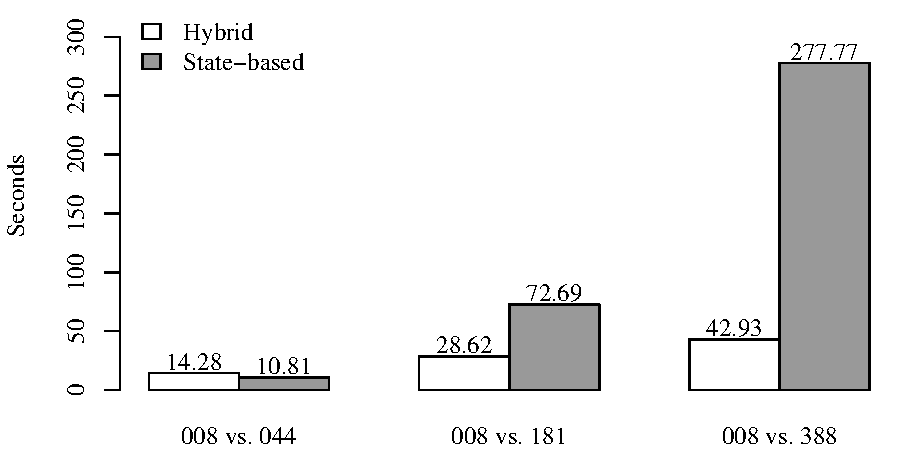
\includegraphics[width=\linewidth]{images/delete_detection_epsilon_average}
    \caption{The time required for hybrid and state-based methods on detecting older version's elements that do not exist in newer versions.}
    \label{fig:delete_detection_epsilon_average}
\end{figure}

For the pair 008 and 044, the change detection is 3.47 seconds faster for the state-based method ($mean$ = 10.81 , $sd$ = 0.16 seconds) than using the hybrid method ($mean$ = 14.28, $sd$ = 0.36 seconds). However, for the pair 008 and 181, the change detection is 44.07 seconds faster for the hybrid method ($mean$ = 28.62 , $sd$ = 0.17 seconds) than the state-based method ($mean$ = 72.69, $sd$ = 1.28 seconds). The hybrid method is again faster for the last pair, 008 and 388: hybrid method ($mean$ = 42.93, $sd$ = 0.18 seconds) is 234.84 seconds faster than the change-based method ($mean$ = 277.77, $sd$ = 4.70 seconds). Considering the increasing number of elements and events (Table \ref{table:version_description}), the change identification time of the hybrid method tends to grow linearly as the number of events increases, whereas the stated-based method tends to grow exponentially as the number of elements increases.

\subsection{Threats to Validity and Limitations}
\label{sec:threats_to_validity_and_limitations}
Since change-based model persistence is a relatively new concept, there are hardly any such models available in public repositories that we could reuse for evaluating our prototype. So far, we have only tested the hybrid model persistence approach on synthesised models which may not be representative of the characteristics of models created by people.

\section{Discussion}
\label{sec:discussion}
The evaluation results for change detection, Section \ref{sec:change_detection}, show that model change detection in hybrid model persistence is substantially faster than state-based comparison. This is because elements and features that have been modified can be directly identified through the events recorded in its CBP representation without the need to compare the models element-by-element. The use of state-based persistence in hybrid model persistence enables faster model loading, as shown by the result of loading time evaluation in Section \ref{sec:model_loading_time}, without having to replay all the changes persisted in its CBP -- the main challenge for the change-based approach \cite{yohannis2018towards,mens2002state}. 
Hybrid model persistence performs slightly slower -- statistically significant for Hybrid XMI but insignificant for Hybrid NeoEMF -- compared to loading a state-based model. A slight slowdown also appears on model saving -- statistically significant for Hybrid XMI but insignificant for Hybrid NeoEMF (Section \ref{sec:model_saving_time}). The slowdown is because changes have to be persisted into two representations, state-based and change-based. 

The main drawback of hybrid model persistence is that it consumes more memory when loading and saving and storage space for persisting models compared to state-based representation only (Sections \ref{sec:model_loading_time}, \ref{sec:model_saving_time}, and \ref{sec:storage_space_usage}). However, considering the cost of main memory and storage, the trade-off can be acceptable in most real-world scenarios.

\section{Related Work}
\label{sec:related_work}
Change-based persistence approaches have been used widely in incremental model management engines (e.g. IncQuery \cite{DBLP:conf/ecmdafa/RathHV12}, ReactiveATL \cite{DBLP:conf/ecmdafa/OgunyomiRK15}) usually by harnessing the notification facilities provided by the underlying modelling framework (e.g. EMF). Such approaches have also been applied in other software \cite{DBLP:journals/entcs/RobbesL07}, databases \cite{DBLP:conf/sde/LippeO92}, hierarchical documents \cite{DBLP:conf/caise/IgnatN05}, model repositories and version control \cite{koegel2010emfstore}. The approach is faster for detecting changes \cite{DBLP:conf/edoc/KoegelHLHD10}, more accurate and carries semantic information (e.g. actors, objects, timestamps, and sequences involved in events) \cite{DBLP:journals/entcs/RobbesL07,DBLP:conf/sde/LippeO92,DBLP:conf/caise/IgnatN05,mens2002state}, faster and more accurate for comparison and merging \cite{DBLP:conf/sde/LippeO92,DBLP:conf/caise/IgnatN05,koegel2010emfstore}, and enable additional analytics activities \cite{DBLP:journals/entcs/RobbesL07}.

There are several non-XMI approaches to state-based model persistence, using relational or NoSQL databases. For example, EMF Teneo \cite{eclipse2017teneo} persists EMF models in relational databases, while Morsa \cite{DBLP:conf/models/Espinazo-PaganCM11} and NeoEMF \cite{daniel2016neoemf} persist models in document and graph databases, respectively. None of these approaches provides built-in support for versioning and models are eventually stored in binary files/folders which are known to be a poor fit for text-oriented version control systems like Git and SVN. Connected Data Objects (CDO) \cite{eclipse2017cdo}, which provides support for database-backed model persistence, also provides collaboration facilities, but CDO adoption necessitates the use of a separate version control system (e.g. a Git repository for code and a CDO repository for models), which introduces fragmentation and administration challenges \cite{barmpis2014evaluation}. Similar challenges arise in relation to other model-specific version control systems such as EMFStore \cite{koegel2010emfstore}. %prefer this to the wording in the repository version!

\section{Conclusions and Future Work}
\label{sec:conlcusions_and_future_work}
In this paper, we have proposed a hybrid model persistence approach and evaluated its impact on time and memory footprint for model loading and saving, storage space usage, and detecting changes of versions of the same model. Based on the evaluation results, the hybrid model persistence provides benefits on model loading time and change detection with an acceptable trade-off on memory footprint and storage space usage.

In the future, we plan to evaluate hybrid model persistence on even larger models and perform experiments where software modellers are asked to construct change-based models. We also plan to develop a solution for efficient merging of change-based and hybrid models. 

\subsubsection*{Acknowledgements.} This work was partly supported by through a scholarship managed by \emph{Lembaga Pengelola Dana Pendidikan Indonesia} (Indonesia Endowment Fund for Education).
%\clearpage
\bibliography{references} 
\bibliographystyle{splncs}

\end{document} 
